\documentclass{article}
\usepackage[utf8]{inputenc}
\usepackage[margin={.95in,.75in}]{geometry}
\usepackage{titlesec}
\usepackage{titling}
\usepackage[default,scale=1]{opensans}
\usepackage{graphicx}
%\graphicspath{ {./} }

\setlength{\parindent}{0em}
\setlength{\parskip}{0.5em}
\renewcommand{\baselinestretch}{1.5}
%\pagenumbering{gobble}

\author{Ryan Bruno}
\date{\today}
\renewcommand{\maketitle}{

\begin{center}
\setlength{\parskip}{0em}
GEOGRAPHY 140:  CULTURAL GEOGRAPHY

Maps and the Media
\end{center}
\textbf{\underline{Name:}}
\theauthor

\textbf{\underline{Title:}}
A Choropleth Map of the Median Household Income in The United States
}

\begin{document}

\maketitle

\textbf{\underline{Analysis}}

\setlength{\parindent}{8ex}
On the next page, I have created a choropleth map showing the median household income in the US. It uses the equal case method meaning each level of income has the same number of states. This is a good method of making choropleth maps however it does not show outliers very well. The map is broken into six levels, with eight states in each. When creating the map I presumed that six gives more detail than four but eight would be too much. With a map like this, we can see patterns that would be hard to see looking at the raw data; let's take a look at some of those patterns.

The first pattern I noticed pertained to the set of top eight states, as they were the first ones I filled in. Seven of the top eight states are located on the east coast; the only exception being California. The last group I drew were the states with the lowest income and they too presented a pattern; all eight of them were in the South. It seems the eastern half of the United States had more income inequality among states then the western half. We can also observe some exceptions that will help with our explanation including Pennsylvania and New York, who both have a lower household income than their neighbors and Georga who have a higher household income higher than its neighbors.

We can explain the high income of some east coast states by looking at their cities. The east coast, uniquely, has many economic centers in a very small area. Boston, New York City, Phillidepha, Baltimore, and D.C. are all large economic centers concentrated in the North East. The low household income of PA and NY can be explained by the amount of rural land they have. Other states in the top eight are small and close to one of the above cities, meaning most of their population is within its economical influence. Conversely, PA and NY are large states with a large proportion of their population living in more rural land outside of the influence of an east coast city, lowering their household income. Moving to the South, we stated it contains all eight of the lowest income level states. There is a historical factor that can explain this. The South started predominantly agricultural, growing cotton and tobacco with the help of African slaves. Meanwhile, the northern states were industrializing. The population in the South was small and after the civil war and emancipation proclamation, it was even smaller. Today, the South is still characterized by its small population and is more rural than the rest of the country explaining its low household income ranking. One exception is Georga. Atlanta's growth has given the South an economical center that may one day be able to compete with its northern counterparts.

The number of categories chosen to create the map proved to work well for our analysis. If I picked four then Georga, Pennsylvania, and New York may have blended in with their neighbors and if I picked eight we may not have been able to notice the income inequality differences between east and west. When reading the map be careful not to confuse light blue and purple; they did not scan well.

%\setlength{\parindent}{0ex}
\begin{figure}[t]
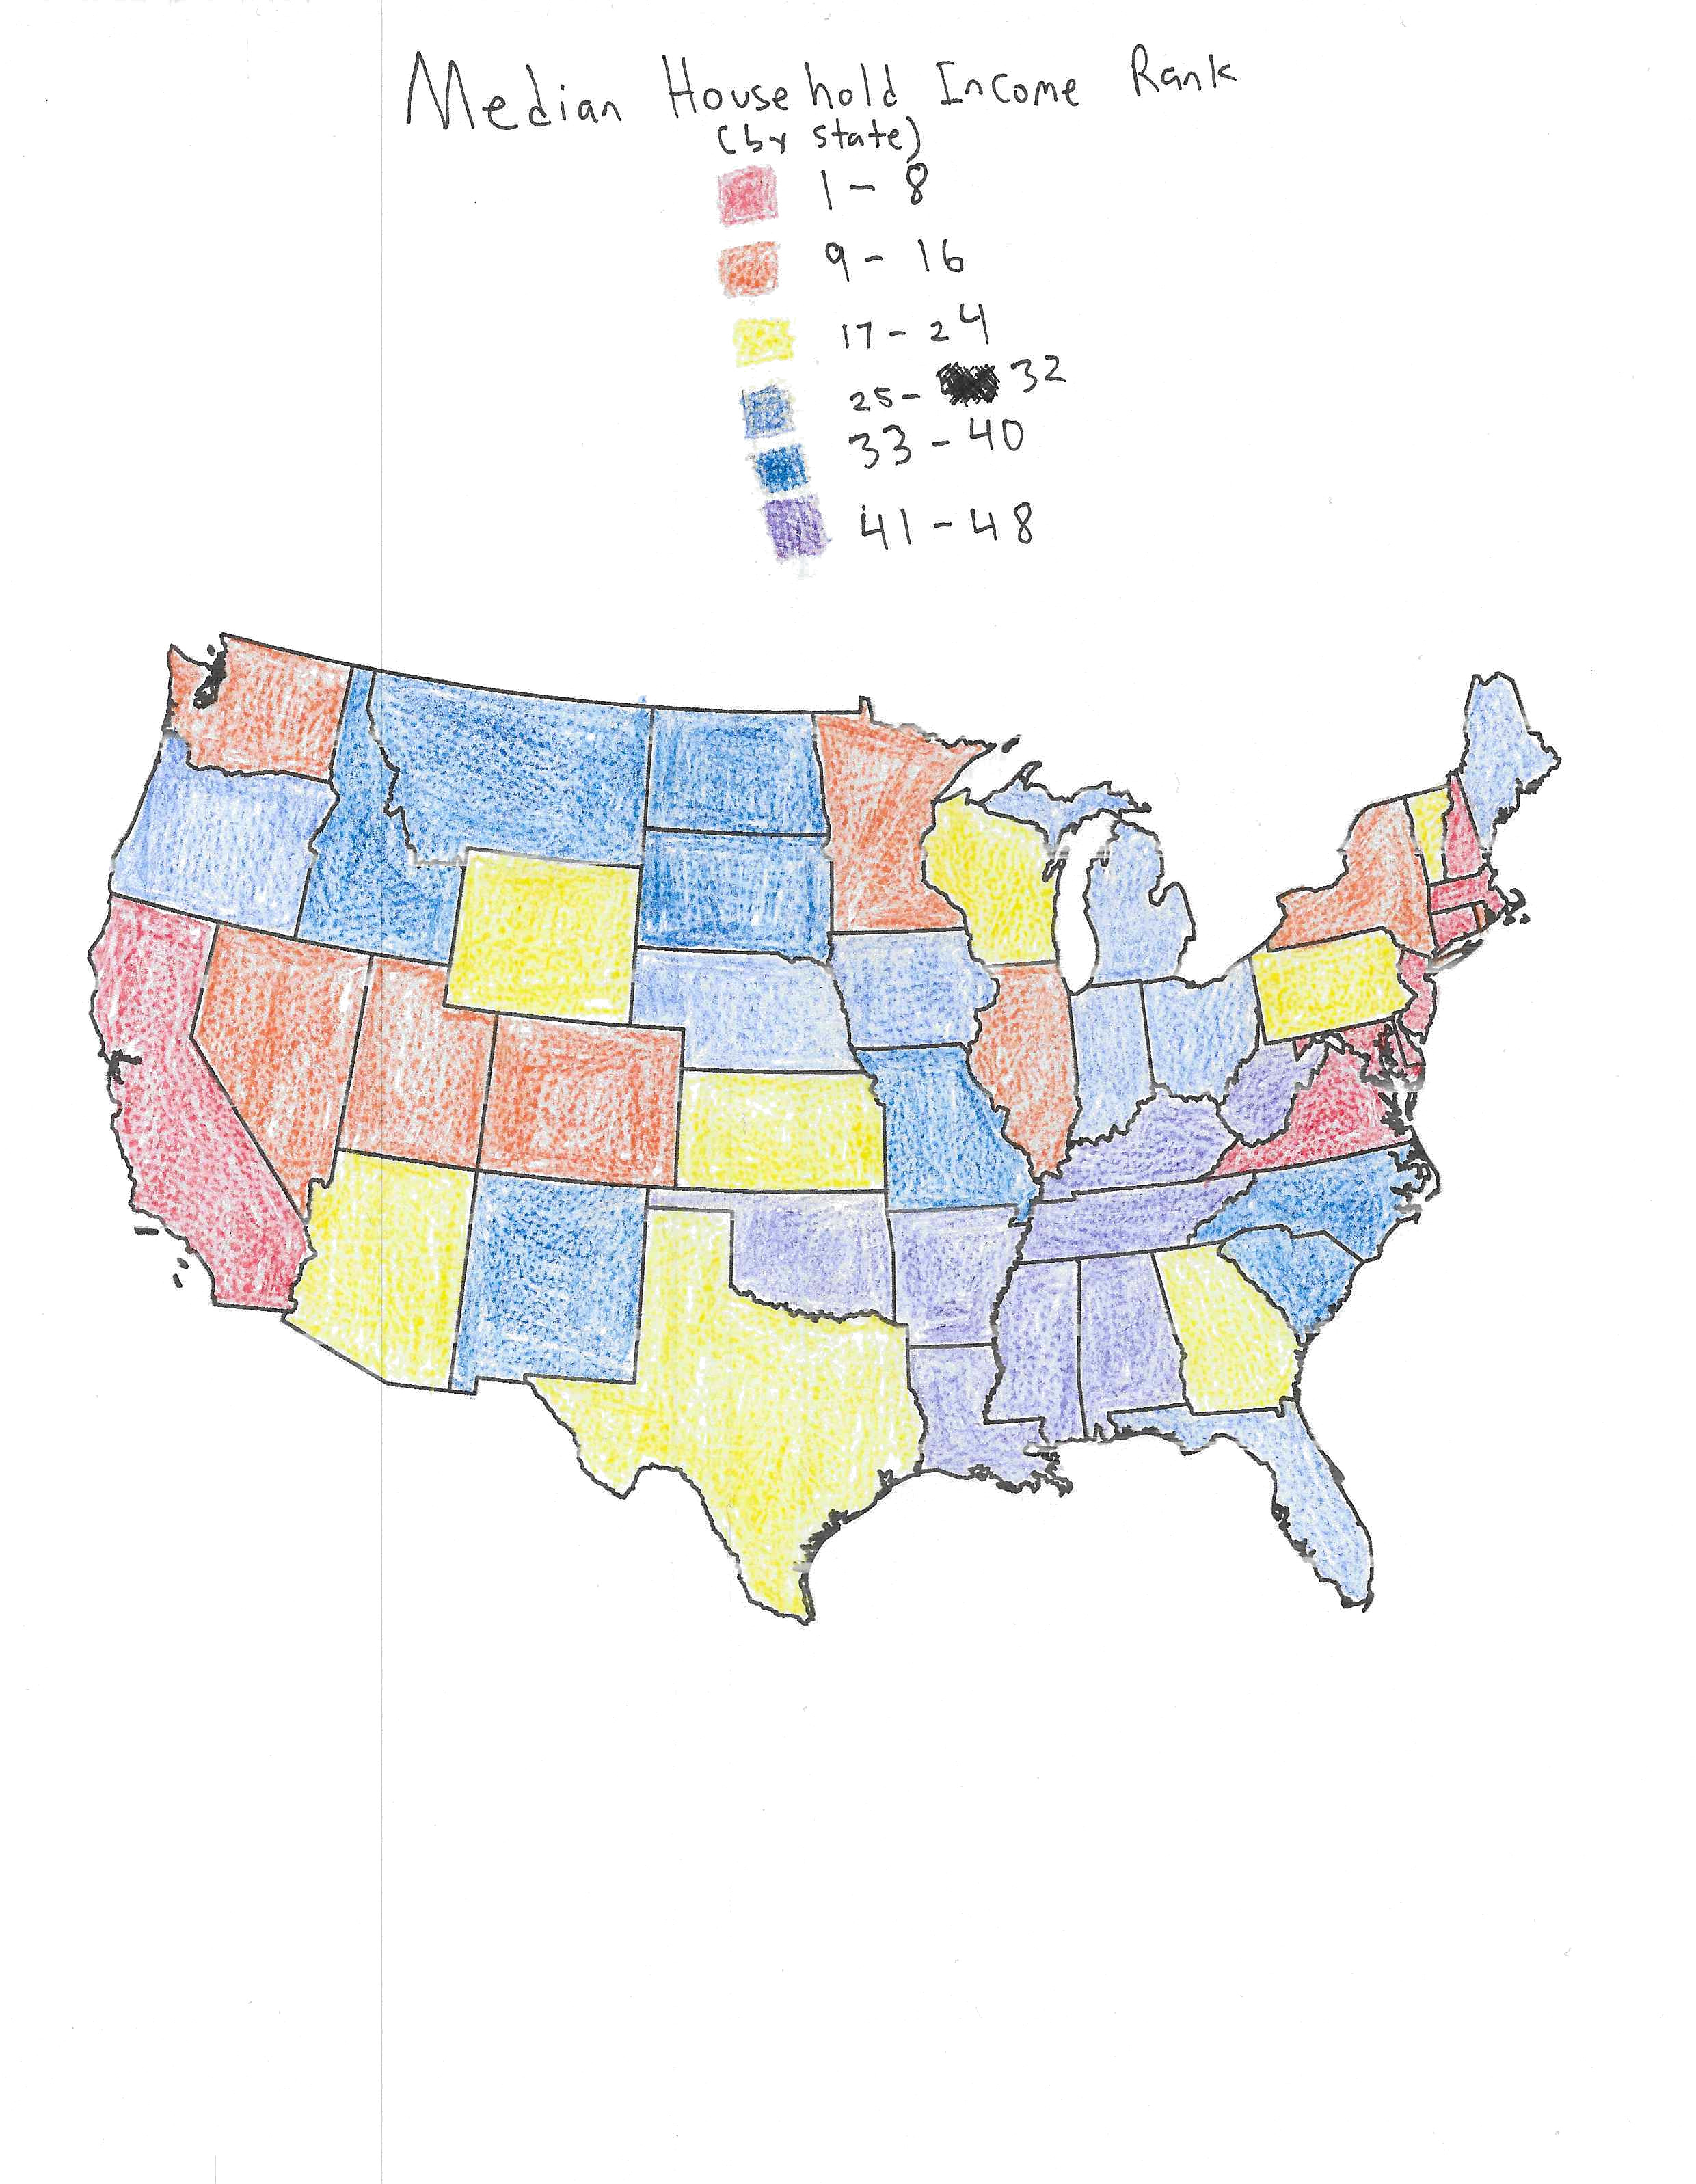
\includegraphics[width=\textwidth]{map}
\end{figure}

\end{document}
